\chapter{Background}
In this chapter we will start by giving an overview of software testing, with particular emphasis on aspects of it that are relevant to this project. We will then take a look at the state of the art in automatic test data generation (ATDG) in order to understand the approach that will be used for \textsf{Flycatcher}. Because the tests will be object-oriented, method call sequences also need to be generated for the test cases and we will look at the state of the art for doing that too. Finally, we will further justify our choice of JavaScript and describe features of it that are of importance for this project.

\section{Dynamic software testing}

\subsection{Overview}

We can define the activity of dynamic testing as testing that requires execution of the software with test data as input \cite{mahmood2007systematic} and characterise it with respect to three parameters namely the amount of knowledge assumed by the tester, the target of the tests and the stage of development at which they are executed. The amount of knowledge of the software under test can be divided into three categories: structural (white-box testing) testing, functional (black-box testing) and a hybrid of the two (grey-box testing). The target of the tests refers to their granularity, from testing specific units of code (unit testing) to an entire integrated system (system testing). The stage at which the tests are undertaken determines whether they are regression tests, alpha-tests, beta-tests, acceptance tests \emph{etc}. With \textsf{Flycatcher}, we generate suites of structural tests, focused at the unit level of object-oriented classes, most likely to perform incremental regression testing. Hence, structural testing, unit testing and regression testing will be described in more detail in this section.

\subsection{Structural testing}

The goal of structural testing is to test the internal workings \cite{mcminn2004search} of an application in order to verify that it does not contain errors. While functional testing determines whether the software provides the required functionality, structural testing tries to ensure that it does not crash under any circumstances, regardless of how it is called. It concerns \emph{how} well the software operates, its structure, rather than \emph{what} it can do, its function. As a result, the measure used to determine good structural testing is the amount of code covered during the testing process --- code coverage. It gives us an \emph{idea} of the amount of code that should be bug free. However, there are various types of code coverage criteria and the confidence that our code is bug free varies depending on which one is chosen.

\subsubsection{Code coverage}
Edvardsson lists the most cited criteria \cite{edvardsson1999survey}, from weakest to strongest:
\begin{itemize}
	\item \textbf{Statement Coverage} Each statement must be executed at least once.
 	\item \textbf{Branch/Decision Coverage} Each branch condition must evaluate to true and false.
 	\item \textbf{Condition/Predicate Coverage} Each clause within each branch condition must evaluate (independently) to true and false.
 	\item \textbf{Multiple-condition Coverage} Each possible combination of truth values for the clauses of each conditional statement must be evaluated.
 	\item \textbf{Path Coverage} Every single path in the control flow graph must be traversed.

%\footnotemark[\value{footnote}
%\footnote{For an explanation of program analysis terminology such as branch, path and control flow graph see Appendix A.}

The stronger criteria of condition, multiple-condition and path coverage are often infeasible to achieve for programs of more than moderate complexity, and thus statement and branch coverage have been recognised as a basic measure for testing \cite{edvardsson1999survey}.
\end{itemize}

\subsection{Unit testing}

Unit testing consists in testing individual and independently testable units of source code \cite{myers2011art}. Therefore, unit testing is made easier if the code is designed in a modular way. The nature of the units depends on the programming language and environment but they are often a class or a function. As opposed to system tests which can be aimed at the client, unit tests are usually white-box tests. Although they do not guarantee that the overall software works as required, they give confidence in specific units of code and narrow down errors, helping the development process. In \textsf{Flycatcher}, the target unit will be \emph{what we will refer to as} a JavaScript `class'. Even though JavaScript does not have a class syntax \emph{per se}, this is what the units will be discussing represent semantically. For clarity we will therefore from this point on use the word `class' to refer to them. Exactly what they are, and how they work, will be introduced later in section~\ref{js}.

\subsection{Regression testing}
Automatically generating structural unit tests can be of great use for regression testing. Regression testing aims to ensure that enhancing a piece of software does not introduce new faults \cite{myers2011art}. The difficulty in testing this is that programmers do not always appreciate the extent of their changes. Hence, having a suite of unit tests with good structural coverage can reduce this problem by verifying the software in a systematic, unbiased way.

\section{Automatic test data generation}
\subsection{Overview}

Although object-oriented test generation requires the creation of objects and method call sequences, it shares with procedural test generation, the need for input \emph{data}. Indeed, the object constructors as well as the method invocations require input parameters, hence Automatic Test Data Generation (ATDG) is a key concern to us. As can be seen in Mahmood's systematic review of ATDG techniques \cite{mahmood2007systematic}, many classifications exist for ATDG techniques. For our purposes, the first distinction that we need to make is between white-box, black-box \cite{prasanna2005survey} and grey-box ATDG techniques, as for \textsf{Flycatcher} we are only interested in white-box testing. In the literature, we found that white-box ATDG techniques are usually classified in two ways \cite{mahmood2007systematic, edvardsson1999survey, tahbildar2automated}:

The first concerns the target selection stage of ATDG techniques: where either paths or individual nodes that contribute to the overall coverage criterion are successively selected from the control flow graph, so that test data that respectively traverses the path or reaches the node can be generated. When specific paths are targeted, the ATDG technique is known as \emph{path-oriented} \cite{edvardsson1999survey} whereas if a node is targeted then it is \emph{goal-oriented}. When data is generated purely randomly \emph{i.e.} there is no specific target, then as part of this classification the ATDG technique is simply \emph{random}.

The other classification of white-box ATDG concerns the type of implementation: \emph{static}, \emph{dynamic} or a \emph{hybrid} of the two \cite{han2008empirical, mcminn2004search}. We will focus on the latter classification of structural testing as it governs our choice of implementation for \textsf{Flycatcher}. Moreover, the former concerns the target selection stage of ATDG and this step will be ignored in \textsf{Flycatcher}, as it is in many recent ATDG techniques \cite{tahbildar2automated}. Figure~\ref{atdg_overview} summarises what we believe is an intuitive characterisation of ATDG techniques with respect to this project and the one which will guide our choice of implementation. Many techniques can be found under each of the static, dynamic and hybrid implementation categories and we will only list the most noteworthy to us.

The choice of implementation for \textsf{Flycatcher} is dynamic random ATDG for our benchmark and dynamic search-based ATDG using genetic algorithms for our solution. The rest of this section will present in further detail the structural ATDG categories and the difficulties of ATDG for a dynamic language, so that we can understand the rationale behind our implementation choice.

\begin{figure}
\hspace*{-1.6cm}
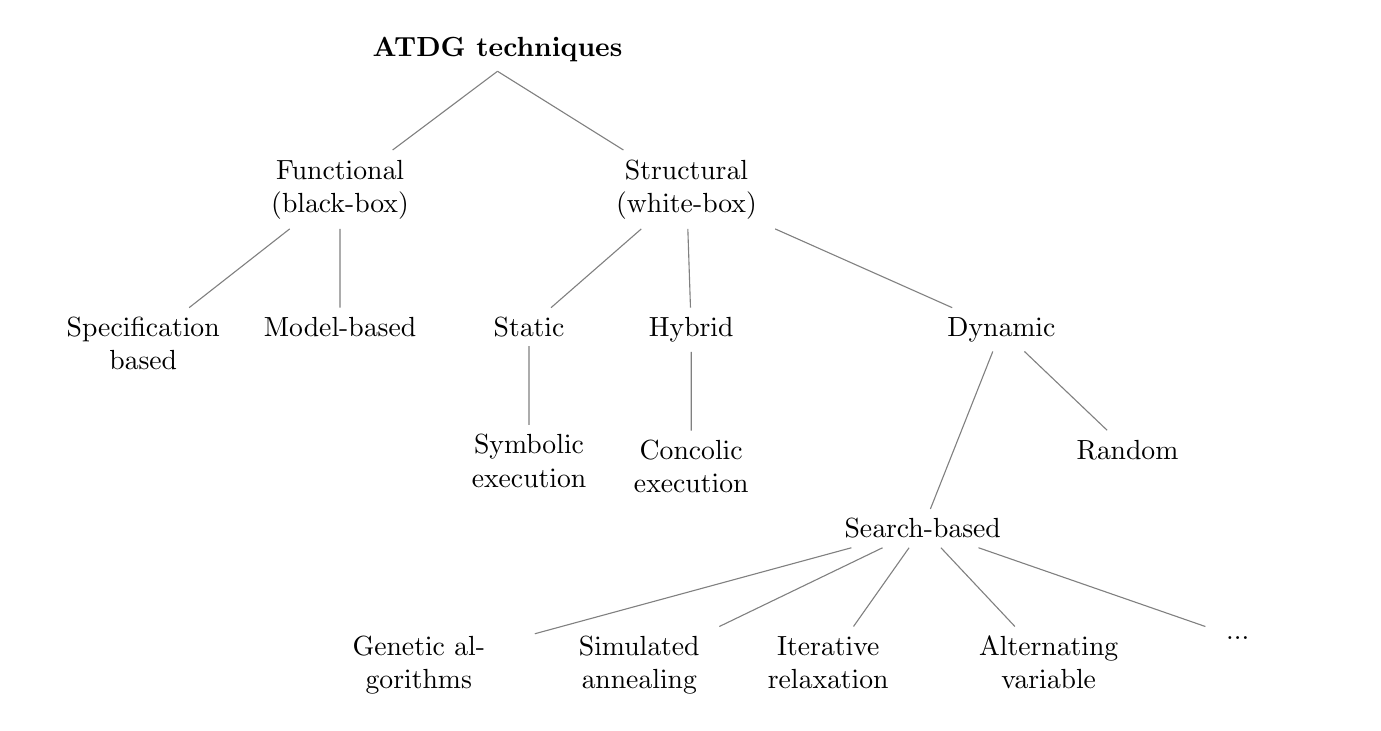
\begin{tikzpicture}[
  	event/.style={text width=2.7cm,text centered,font=\rmfamily,anchor=north},
  	edge from parent/.style={draw=black!50},
   % 	edge from parent path={(\tikzparentnode.south) -- ++(0,-0.5cm)
	%		-| (\tikzchildnode.north)},
	level 1/.style={sibling distance=4cm,level distance=1cm,
		growth parent anchor=south,nodes=event},
	level 2/.style={sibling distance=4cm},
	level 3/.style={sibling distance=4cm},
	level 4/.style={sibling distance=4cm}]

	\node {\textbf{ATDG techniques}}
		child [yshift=1cm] {
			child {node [level 1] {Functional (black-box)}
				child {node [level 2, xshift=-0.5cm] {Specification based}}
				child {node [level 2, xshift=-2cm] {Model-based}}
			}
			child {node [level 1,xshift=0.4cm] {Structural (white-box)}
				child {node [level 2,xshift=2cm] {Static}
		     	       child {node [level 3] {Symbolic execution}}}
				child {node [level 2,xshift=0.06cm] {Hybrid}
						 child {node [level 3] {Concolic execution}}}
				child {node [level 2] {Dynamic}
	    	 	      child {node [level 3,text width=2.5cm,xshift=1cm,yshift=-1cm] {Search-based}
			      		child { node [level 4,xshift=1.6cm] {Genetic algorithms}}
			      		child { node [level 4,xshift=0.4cm] {Simulated annealing}}
			      		child { node [level 4,xshift=-1.2cm] {Iterative relaxation}}
							child { node [level 4,xshift=-2.4cm] {Alternating variable}}
							child { node [level 4,xshift=-4cm] {...}}
			      }
		     	      child {node [level 3,text width=2.5cm,xshift=-0.4cm] {Random}}
				}
			}
		};
\end{tikzpicture}
\caption{Overview of ATDG techniques}
\label{atdg_overview}
\end{figure}


%We feel that the latter is more intuitive as specific ATDG techniques usually fall under one of these categories. Figure 123 summarises what we believe is the most intuitive characterisation of ATDG techniques to date and the one which will guide our choice of implementation for \textsf{Flycatcher}.

%Edvardssvon's classification \cite{edvardsson1999survey} is based on the idea that there are three approaches to automatic test data generation. The idea is that . Once a path is chosen it can be traversed by three methods: \emph{random}, (randomly explore the search space) \emph{goal-oriented} (target specific goals such as assertions) and \emph{path-oriented} (traverse an exact path).

\subsection{Static test data generation}
Static structural test data generation is based on information available from the static analysis of a program, without requiring that the program be actually executed \cite{mcminn2004search}. Static program analysis produces control flow information that can be used to select specific execution paths in order to try and achieve good coverage. The goal of ATDG is then to generate data that executes these paths.

Every time control flow branches, \emph{e.g.} at \texttt{if} statements, there is a corresponding predicate or branch condition. These predicates can be collected along a path and conjoined to form the path predicate. By solving the path predicate in terms of the input variables, we can obtain test data that executes that path. However, in order to rewrite the path predicate in terms of the input variables we need to take into account the execution of the program. Hence, to generate the test data statically a technique called symbolic execution \cite{king1976symbolic} is used.

Symbolic execution gathers constraints along a simulated execution of a program path, where symbolic variables are used instead of actual values, such that the final path predicate can be rewritten in terms of the input variables. Solving the resulting system of constraints then yields the data necessary for the traversal of the given path \cite{king1975new, king1976symbolic}. There are a lot of technical difficulties associated with symbolic execution \cite{edvardsson1999survey,meudec2001atgen,mcminn2004search}:

%\renewcommand{\labelitemi}{\tiny$\blacksquare$}

\begin{itemize}
	\item the presence of input variable dependent loops can lead to infinite execution trees\footnote{the execution paths followed during the symbolic execution of a procedure \cite{king1976symbolic}} as the loops can be executed any number of times
	\item array references become problematic if the indexes are not constants but variables, as is typically the case
	\item features such as pointers and dynamically-allocated objects that rely on execution are hard to analyse statically
	\item static analysis is not possible for function calls to precompiled modules or libraries
	\item if the path constraint is non-linear, solving it is an undecidable problem
	\item even if the path constraint is linear, solving it can lead to very high complexity
\end{itemize}

Although various static solutions have been proposed for these issues \cite{ramamoorthy1976automated,goldberg1994applications,offutt1999dynamic}, they often dramatically increase the complexity of the ATDG process. As a result, tools purely based on symbolic execution can typically handle only subsets of programming languages and are not applicable in industry. A better trend that has developed in the past decade, is the combination of concrete and symbolic execution, which tackles most of the aforementioned issues \cite{păsăreanu2009survey} --- we will cover this type of ATDG implementation in~\ref{subsec:hybrid_atdg}. Due to the numerous problems posed by purely static ATDG, its weakness with dynamic types and constructs \cite{edvardsson1999survey,tahbildar2automated} and the complexity of building a fully-fledged symbolic executor for a language \cite{edvardsson1999survey,han2008empirical}, we chose not to use static ATDG for the implementation of \textsf{Flycatcher}.

\subsection{Hybrid test data generation}
\label{subsec:hybrid_atdg}

The hybrid approach to ATDG consists in combining symbolic and concrete execution, which is known as \emph{concolic execution} \cite{păsăreanu2009survey}. In other words, hybrid analysis tools run programs on actual inputs, while collecting symbolic constraints in order to direct the search for new inputs. In doing so, they avoid the main weaknesses of the static approach, such as solving non-linear constraints or dealing with dynamic structures --- the concrete inputs are used when need be. This type of technique has been popular in recent years, mainly because it overcame the limitations that prevented static ATDG techniques from being applied to industry software. Notable tools that implement it are DART \cite{godefroid2005dart}, CUTE \cite{sen2005cute}, JPF-SE \cite{anand2007jpf}, PEX \cite{tillmann2008pex}, EXE \cite{cadar2008exe} and KLEE \cite{cadar2008klee}.

Yet, although hybrid ATDG deals with some limitations of static ATDG, the constraint-solving based approach that hybrid ATDG also employs is impractical for generating \emph{complex} input data. Additionally, the highly dynamic nature of JavaScript makes it very difficult to infer any information from the program statically. Hence, hybrid analysis, as it relies on static symbolic execution, is not adequate either for our purposes.

\subsection{Dynamic test data generation}

Dynamic test data generation is purely based on actual execution of the software. The program under test is run with, possibly randomly, selected input and feedback is collected at runtime regarding the chosen coverage objective \cite{edvardsson1999survey}. The feedback is usually obtained through some form of instrumentation of the program that monitors the program flow. Inputs can be continually generated randomly, relying on probability to achieve the coverage objective --- this is known as \emph{random} test data generation and does not perform well in general \cite{edvardsson1999survey}. On the other hand, inputs can be incrementally tuned based on the feedback (using different kinds of search methods) in order to satisfy the coverage objective --- this is known as \emph{search-based} test data generation \cite{mcminn2004search}, where the search-space is the control flow graph of a program. The main drawback of dynamic ATDG is that it is reliant on the speed of execution of a program and as the number of required executions to achieve satisfactory coverage may be high, this leads to an overall expensive process. Below we will present the random and search-based approaches in more detail, in order to understand which would be more suitable for \textsf{Flycatcher}.

\subsubsection{Random approach}

Random test data generation consists in producing inputs at random in the hope of achieving the chosen coverage criterion through probability. Although random test data generation is relatively simple to implement, it does not perform well in terms of coverage, as the chances of finding faults that are revealed by only a small percentage of program inputs are low \cite{edvardsson1999survey}. In other words, it is difficult for it to exercise `deep' features of a program that are exercised only through specific and unlikely paths. As a result, random ATDG only works well for straightforward programs. However, because it is the simplest ATDG technique and is considered to have the lowest acceptance rate \cite{edvardsson1999survey}, it is often used as a benchmark and is a suitable candidate for us to benchmark our \textsf{Flycatcher} application.

\subsubsection{Search-based approach}
% more on search-based approach using mairhofer's stuff?

Search-based test data generation uses heuristics to guide the generation of input data so that the inputs execute paths that contribute to the overall test coverage objective. This involves modelling the test coverage objective as a heuristic function or \emph{objective function}, that evaluates the fitness of a chosen set of inputs with respect to a coverage objective. Based on those fitness values, many search techniques exist to find optimal inputs in order to achieve the desired coverage. Various objective functions exist and they are dependent on the ATDG method used. Some of the well-known search-based ATDG techniques are \emph{alternating variable} (local search optimisation) \cite{korel1990automated, gallagher1997adtest}, \emph{simulated annealing} \cite{tracey1998automated,tracey1998way}, \emph{iterative relaxation} \cite{gupta1998automated} and \emph{genetic algorithms} \cite{michael1998automated,michael2001generating}.
 
In 2008, Han and Kwon \cite{han2008empirical} conducted a robust empirical evaluation of search-based test data generation techniques, comparing iterative-relaxation, local search optimisation and genetic algorithms. Genetic algorithms came out on top of the other techniques regarding the rate of coverage and generality, both essential characteristics when considering ATDG techniques. However, genetic algorithms proved expensive both in time and resources, but this can be improved upon \cite{han2008empirical}.
Although simulated annealing is not part of this empirical evaluation, we can see from \cite{michael1998automated} that although it performs as well as genetic algorithms, it appears to be less efficient.

Additionally, genetic algorithms offer another advantage: as opposed to most other ATDG techniques, they do not require static analysis of the program under test \cite{han2008empirical}. This advantage is especially significant in our case, as to the best of our knowledge, tools that produce control and data flow analysis information for JavaScript source code are not available. However, this is not surprising since the dynamic, object-oriented nature of JavaScript makes this task very laborious.

Consequently, due to their effectiveness in terms of coverage and the advantages they possess with regard to dynamic languages, genetic algorithms appear to be the most suitable for our implementation of ATDG for \textsf{Flycatcher}. We will therefore go on to explain what genetic algorithms are and how they can be applied to test data generation.

\subsection{Genetic algorithms}

\subsubsection{Overview}
Genetic algorithms attempt to model the robustness and flexibility of natural selection in order to guide a search \cite{michael2001generating}. They start with a randomly initialised \emph{population} of potential candidate solutions, called \emph{individuals} or \emph{chromosomes}. The population is iteratively recombined and mutated to evolve successive populations, known as \emph{generations}. The recombination takes the `fittest' parent solutions and `breeds' them to produce new offspring. Their fitness is determined by a \emph{fitness function} that evaluates how good a candidate solution is for a particular problem.

This process favours evolution towards fitter individuals, mimicking natural selection. The `breeding' of two individuals usually involves a \emph{crossover} operation which swaps their information at a randomly selected position. In the interest of maintaining diversification, a \emph{mutation} phase usually occurs after the crossover, to introduce new genetic material into the search and avoid premature convergence on one area of the search space. The mutation operation randomly modifies some information of a selected individual. The process of iterative recombination and mutation, illustrated in Figure \ref{ga}, is repeated until a specific termination criterion is fulfilled.

\begin{figure}
\hspace*{0.7cm}
\centering
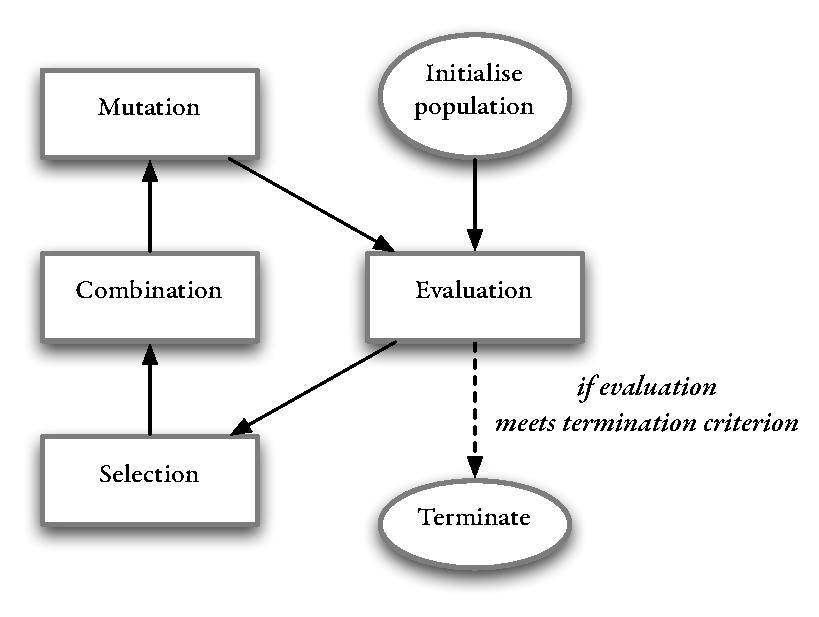
\includegraphics[scale=0.7]{./components/chapter2/ga.pdf}
\caption{Flowchart of a genetic algorithm}
\label{ga}
\end{figure}

\subsubsection{Application to test data generation}
\label{subsubsec:ga_application}
For the purposes of ATDG, the population consists of input test data. The data evolves according to the genetic algorithm in order to satisfy the chosen coverage criteria \cite{michael2001generating}. In other words, the \emph{fitness function} is based on the \emph{objective function}, the function that evaluates test data according to a certain coverage criterion --- the more a candidate contributes to coverage, the fitter it is. Instead of using a search heuristics to minimise our objective function, we use it to guide our natural selection process towards the data that will achieve the best coverage.

Regarding the objective function used in the context of genetic algorithms, different variants exist \cite{mcminn2004search}. The \emph{coverage-oriented approach} rewards individuals on the basis of \emph{all} covered program structures. This type of objective function rewards coverage with respect to the overall goal \emph{i.e.} the system is not required to pick a specific path or node and attempt to execute it. The other approach is \emph{structure-oriented} coverage where, similarly to most other search-based ATDG methods, a structure (\emph{e.g.} a path or a node) is selected from the data flow analysis and a separate search is undertaken for each selected structure. Once more, seeing that the \emph{coverage-oriented approach} does not require static analysis of the program under test, it is the most attractive to us for the implementation of \textsf{Flycatcher}.

Finally, the population, individual representation, fitness evaluation and methods of crossover, mutation and selection are all highly dependent on the test data generation problem at hand, hence we will discuss them with regard to \textsf{Flycatcher} when we come to the implementation.

%For a simple procedural language the evolution process will deal with test data whereas for object-oriented tests, the recombination and mutation could concern call sequences and types.

%We believe that obtaining the best coverage for possibly complex programs is worth using GA. GA does not 

% tends to be as effective in terms of coverage, the simulated annealing method requires more executions than the GA method and is therefore less desirable. Additionally -> less work for GA implementation = no static analysis information needed? no instrumentation needed? 

%The iterative-relaxation method is part of the hybrid approach and we will look at this type of approach later in the next section. Regarding the search-based methods which are part of the dynamic approach to ATDG,

%through the program execution search-space in order to achieve the chosen test coverage criteria.

\subsection{Challenges of dynamic languages}

Most of the research on ATDG so far concerns static programming languages \cite{mahmood2007systematic} and it is only in the past few years that dynamic programming languages have sparked some interest in that field. A possible reason for this is that dynamic programming languages make ATDG \emph{harder} by enabling features that allow programs to significantly change at runtime. These features can include modifying the type system, extending objects or adding new code, all during program execution. The challenges that this type of behaviour introduces for ATDG are listed below \cite{ducasse2011challenges}.

\subsubsection{Generating test data of the required type}
Given that method parameters do not have static types in dynamically typed languages, we do not know what arguments to pass to them. A potential solution to this is to use a method called \emph{type inference} \cite{pluquet2009fast}, which tries to infer the type of arguments from the way they are used inside the program. Although this method does not guarantee 100\% precision, it is a good starting point for generating accurately typed test data in a dynamic setting. Mairhofer uses this technique for \textsc{\small RuTeG} \cite{mairhofer2008search}, his search-based ATDG tool for Ruby, where the search for test data refines the initially inferred type, by discarding poor candidates. We will inspire ourselves from this approach.

\subsubsection{Generating object instances}
Sometimes input parameters will be of a complex type and this complicates the test data generation task even further. Generating well-formed object instances to use as arguments inside tests for a dynamically-typed object-oriented language is problematic because there isn't a blueprint to construct them from. There is previous work on input data generation for dynamic data structures \cite{korel1990automated, visvanathan2002generating, sai2005address, zhao2007automatic}, but all these approaches focus on statically typed languages (C/C++), require static program analysis and mostly lack generality.

Another approach uses needed-narrowing \cite{antoy1994needed} or lazy instantiation \cite{lindblad2007property} --- where instances are created empty and their members are only created when they are actually put to use by the program. This enables test case generators to adjust object instances during execution, when attempts are made to use them, so that they always have the required type. This technique is used by \textsc{Irulan} \cite{allwood2011high} for generating tests in Haskell, which has lazy evaluation by default. For the purpose of complex type test data generation in \textsf{Flycatcher}, we will use a different method but the idea of returning adequate objects upon their use in the program will be present.

\subsubsection{Identifying bugs}

In dynamic languages such as JavaScript, the function signatures bear no type information. This makes it difficult to know whether an exception is raised due to a wrongly typed test argument or a true program bug.

In the case where the exception is not a bug it could be due to two things: manipulating a badly initialised object or breaking a program precondition. The former can be avoided by ensuring correct parameters are passed to object constructors \emph{i.e.} the crux of this project. The latter can be solved by giving the tester the ability to impose restrictions on the test data generator, so that preconditions for the program are respected.

As for real software errors, \textsf{Flycatcher} will deal with those too, and this matter will be revisited later.

\subsubsection{Dealing with dynamically generated code}

Dynamic languages sometimes offer features that parse and evaluate a string at runtime and execute it as code, such as JavaScript's \texttt{eval} function. However, not only are these features potentially insecure, they make any analysis for test data generation much harder. As the general use of \texttt{eval} in JavaScript is prohibited anyway\footnote{\tiny"\url{https://developer.mozilla.org/en/JavaScript/Reference/Global_Objects/eval#Don't_use_eval!}"}, we can safely ignore it for the purpose of our application.

\section{Object-oriented test case generation}
Most of the research on test generation focuses on testing imperative functions, such that the automated generation required is that of the functions' input parameters. However, when dealing with object-oriented code, a different approach is needed, as the unit under test changes from a function to an object. To test one of an object's methods, three steps are necessary \cite{tonella2004evolutionary} and should be repeated until the chosen coverage criterion for the method under test is met.
\begin{enumerate}
	\item Instantiate the object
	\item Call some of its methods to possibly modify its state
	\item Assert that the method under test returns the expected answer
\end{enumerate}

Because it is impossible to know how the application will use the class/object under test in practice, as many relevant test cases as possible must be tried in order to maximise the likelihood of finding a bug inside the class in question. Coverage, the assessment measure that is often used for test \emph{data} generation, is an equally good indicator of the relevance of test \emph{cases}. Hence, this measure can be used, as for the generation of input \emph{data}, as a search objective to guide the generation of \emph{method call sequences} for our test cases. Tonella was one of the first to use search-based methods for the generation of adequate object-oriented test cases, using genetic algorithms as the search heuristics method \cite{tonella2004evolutionary}. Indeed, the procedure of using genetic algorithms to generate input test data for \textsf{Flycatcher} described in~\ref{subsubsec:ga_application} can simply be extended to the generation of object-oriented tests by adapting individuals so that they represent the structure of a test case.

The code example below illustrates in pseudocode the type of object-oriented structural unit test that we aim to generate with \textsf{Flycatcher}. It assumes a standard linked list implementation, \texttt{LinkedList} is the class under test and \texttt{size} is the method under test:

\begin{verbcode}
l = new LinkedList   
node = new Node
l.add(node)
l.remove(node)
l.add(node)
assert (l.size == 1)
\end{verbcode}

%, as well as their inputs and the inputs to the constructor, should all evolve in a way that permits a successful coverage to be achieved. Automatic test \emph{data} generation techniques that maximise coverage have been discussed, but work has also been done on techniques to the evolution of object-oriented tests cases.

%One thing to note about such a test case is that it does not mean the method under test is bug-free --- again, the unit under test is the object, therefore many instantiations and method call sequences need to be tried
%One element of this procedure that we have not discussed so far is the generation of a sequence of method calls for the second step.

%create a sequence of methods leading to the method under test, it is the method under test which gives an assertion using its return value

\section{JavaScript}

\subsection{Why JavaScript?}

With cloud computing and the ubiquitous shift of desktop applications to the web, web development has taken on a whole new meaning. Along with this shift, the languages of the web have become much more significant to the software world. JavaScript particularly so, due to its powerful multi-paradigm nature (and despite its unanimously condemned defects). As a result, while in the past JavaScript was used for no more than to animate static HTML pages, today it powers 3D game engines and other fast real-time applications on the web. On top of its pervasiveness on the client-side of the web, it has now also reached web servers and desktop scripting environments.

The move that JavaScript seems to be making from the world of scripts to the world of applications means that it is used in more complex and modular code. This in turn comes with the need to test those applications using standard software techniques: unit testing, regression testing \emph{etc.} Due to the relative recency of the surge in popularity of JavaScript, which can be observed in Figure \ref{TIOBEgraph}, no effort has yet been made to automate its testing effort. This is where \textsf{Flycatcher} can make a difference, and this is why JavaScript was chosen for this project: JavaScript is on its way up and there is an opportunity to help its growing community of developers.

\begin{figure}
\hspace*{-1.2cm}
\centering
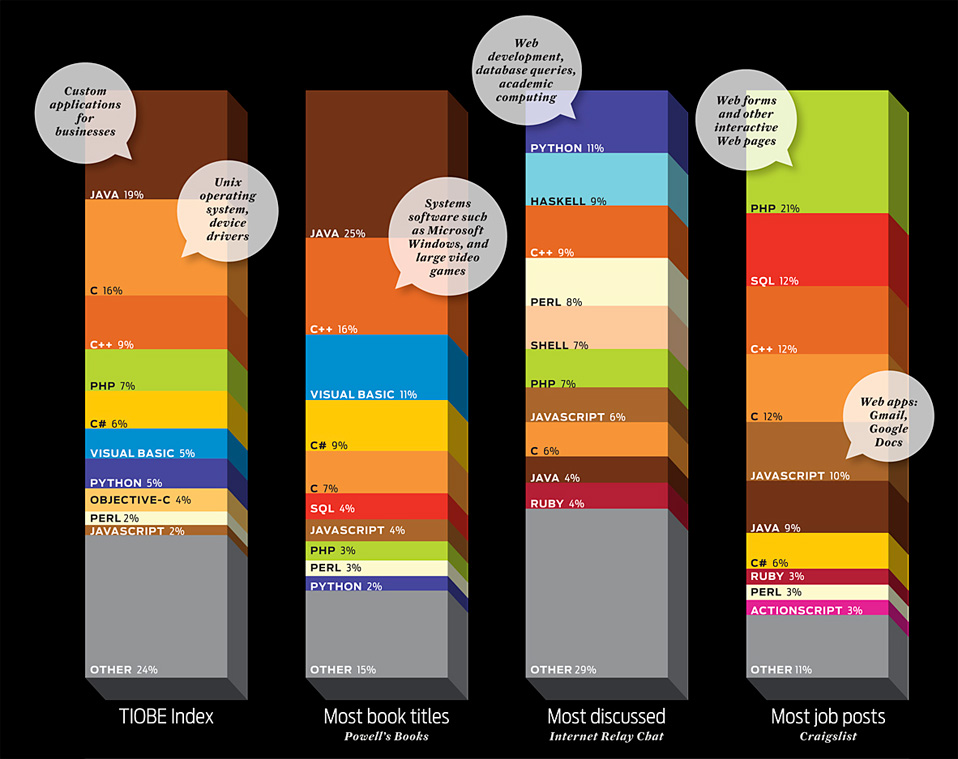
\includegraphics[scale=0.45]{./components/chapter2/TIOBEgraph.jpeg}
\caption{The top 10 programming languages 2011 \cite{tiobe}}
\label{TIOBEgraph}
\end{figure}

\subsection{Overview}

JavaScript is a dynamic scripting language with weak, duck typing and first-class functions. It is multi-paradigm, supporting imperative and functional styles, as well as object-oriented programming through the use of objects and object prototypes. When used specifically within browsers, JavaScript programs come with certain characteristics, but since we are targeting a wider range of programs, we will focus on the core of the language, as specified by the ECMA-262 5.1 edition standard\footnote{http://www.ecma-international.org/publications/files/ECMA-ST/Ecma-262.pdf} --- although given the time constraints, we will work with a subset of it.

\subsection{Idiosyncratic features}
For the readers who are not familiar with the language, we present the characteristic features of JavaScript \cite{flanagan2006javascript} that are important in this project.

\subsubsection{Types}
Types in Javascript can be divided into two categories: \emph{primitive} types and \emph{object} types. The primitive types consist of \emph{Number}, \emph{Boolean} and \emph{String}, as well as \texttt{undefined} and \texttt{null} but the latter are particular as they are the only element of their type. Anything else in JavaScript will have the type \emph{Object} (even arrays and functions). Generally, a JavaScript object is an unordered collection of named values, \emph{properties}, that can be stored or retrieved by name \emph{e.g.}:

\begin{verbcode}
var foobar = { `foo' : 1,
               `bar' : 2 };
foobar.foo     // returns 1
foobar[`bar']  // returns 2
foobar.bar = 3
foobar.bar     // returns 3
\end{verbcode}

JavaScript also has specialised objects, such as \emph{Arrays} and \emph{Functions}. Arrays are untyped, ordered collections of elements (primitives or objects) that can be accessed through a numerical index. Although arrays exhibit additional behaviour, they \emph{can} be thought of as mere objects whose properties happen to be integers.

Functions however, although they are treated as first-class objects and can be stored in variables, differ significantly. They are defined as code blocks with parameters, local scope, an invocation context \texttt{this} and may return a value if invoked. Below are examples of a JavaScript function definition:

\begin{verbcode}
function add(a,b) {
    return a + b;
}
\end{verbcode}
\noindent \emph{or} equivalently:

\begin{verbcode}
var add = function(a,b) {
    return a + b;
}
\end{verbcode}

An important feature of JavaScript is that it is dynamically typed, hence a variable cannot imply a type for its value and its type can change over time \emph{i.e.} the code below is correct:

\begin{verbcode}
var foo = "foo?";
foo = 3;
foo = [1,2,3];
foo = function() {return "foo!"};
foo(); // returns "foo!"
\end{verbcode}

Equally, the function \texttt{add} defined earlier does not imply any types for its parameters, it could well be a function that concatenates two strings for instance. Although JavaScript supports the object-oriented paradigm, the way it does so is quite different from most object-oriented languages and we will see that functions play a central role.

\subsubsection{Object-oriented programming}
\label{js}

JavaScript is known as a \emph{prototype-based} language, meaning that it does not have traditional class definitions to represent object blueprints and create instances of them, but rather that object instances can be used as prototypes to construct other objects instances. That way, we can say, tying this back to classical OOP, that if two objects inherit properties from the same prototype object, they are instances of the same class. The role that functions have in this is that, usually, if two objects inherit properties from the same prototype object, it means that they have been created and initialised by the same function --- this function is known as their \emph{constructor}.

A constructor is a function typically \emph{designed} for the initialisation of newly created objects. When called with the keyword \texttt{new}, its invocation context represents the object being created, hence it can initialise the object's properties by using the \texttt{this} keyword and then return it as the newly created object. A key feature of constructors is that their \texttt{prototype} property (an object) is also used to initialise the object they construct --- the new object \emph{inherits} from the prototype object which is why it is called prototypical inheritance.

To summarise, a class in JavaScript is defined by a constructor function\footnote{which is not technically different from standard functions except that it is \emph{intended} to be called with the \texttt{new} keyword} through two elements:

\begin{enumerate}
   \item its body, which initialises objects through accessing \texttt{this} (the class fields are defined here)
   \item its \texttt{prototype} property, from which the constructed objects inherit all properties (the class methods are defined here)
\end{enumerate}

Below is an example of a simple class definition for a circle, to illustrate our explanation:

\begin{verbcode}
function Circle(radius) {
    // the Circle class has a field named radius
    this.radius = radius;
}

// the Circle class has a method getCircumference
Circle.prototype.getCircumference = function() {
    return this.radius * Math.PI * 2;
}

var c1 = new Circle(1);
var c2 = new Circle(2);

c1.getCircumference() // returns approx. 6.28
c2.getCircumference() // returns approx. 12.56

\end{verbcode}

In the example above, note that the invocation context of the constructor is returned automatically when the constructor is called with the keyword \texttt{new}. Also, both \texttt{c1} and \texttt{c2} have a \texttt{radius} field (though initialised to different values) and a \texttt{getCircumference} method, as they were initialised with the same constructor --- we can say that they have the same `class'. In \textsf{Flycatcher}, classes are what we will use as the target unit for generating suites of unit tests and this is what we will be referring to.

Finally, although classical OOP techniques such as subclassing, polymorphism and encapsulation are all possible in JavaScript, they are not a key concern to us and we will ignore them at this stage.

\subsection{Harmony}
The JavaScript language and its derivatives JScript, ActionScript \emph{etc.} were formalised in 1997 by Ecma International under the name ECMAScript. The ECMAScript specification, namely ECMA-262, standardises the core of the JavaScript language and thus serves as a common ground for its implementation. The latest published version of the standard is edition 5, which is implemented in all major browsers.

Nevertheless, there is a very interesting and landmark edition in progress called \emph{Harmony}, with many new exciting language features. Among those features is a meta-programming API, which, although currently non-standard, is already implemented by major browser engines such as Google's V8 engine and Firefox's SpiderMonkey. The meta-programming API presents a new type of object which is extremely powerful and helpful for the development of \textsf{Flycatcher}: the \emph{Proxy} object.

\subsubsection{Object Proxies}
Proxies are special objects that let the programmer define the \emph{behaviour} of an object \emph{i.e.} how it responds to low-level operations. This is done through a `catch-all' mechanism, which \emph{traps} or \emph{intercepts} low-level operations on the proxy and allows us to redefine their outcome. To illustrate this, we define a simple Proxy that overrides the \texttt{[[Get]]} low-level operation and traps property accesses of the form \texttt{proxy.name} in the context of \emph{getting} a property's value. We override that behaviour and return the string \texttt{''It's a trap!''} instead:

\begin{verbcode}

var proxy = Proxy.create({
  get: function(receiver, name) {
    return name + '' -> It's a trap!'';
  }
});

proxy.treasure = ''gold'';
proxy.treasure // returns ''treasure -> It's a trap!''
\end{verbcode}

The \texttt{receiver} is a handle to the proxy itself, and the \texttt{name} is the name of the property being trapped. The object passed to the Proxy's \texttt{create} function is called its handler and needs to implement a specific API, so that all of the fundamental low-level operations on the object respond, but it is not necessary to detail it here. It is worth noting about Proxies, as this will matter to us later, that some operations are not trapped in order to respect the language invariants:

\begin{itemize}
   \item The tripple equal \texttt{===} operator isn't trapped \emph{i.e.} \texttt{p1 === p2} \emph{only} if \texttt{p1} and \texttt{p2} are a reference to the same Proxy object
   \item The \texttt{typeof} operator
   \item The \texttt{instanceof} operator
   \item The \texttt{Object.getPrototypeOf(proxy)} operation
\end{itemize}

There is much more to say about object Proxies and their applications, but this brief introduction is sufficient in our case.

\subsubsection{Function Proxies}

Harmony also proposes \emph{function} Proxies, which are useful to us. Functions in JavaScript are objects, hence, function Proxies have the \emph{same} trapping capabilities but they also offer \emph{additional} traps, which are specific to functions: the \texttt{call} trap and the \texttt{construct} trap. To illustrate we give an example of a function proxy in action:

\begin{verbcode}

// handler is as earlier, construct and call are functions
var fnproxy = Proxy.create(handler, call, construct);
fnproxy.treasure   // calls handler.get(fnproxy, treasure)
fnproxy(1,2,3)     // calls call(1,2,3)
new fnproxy(1,2,3) // calls new construct(1,2,3)

\end{verbcode}

\section{Summary}

Despite being tedious and prone to human error, testing is a necessary and important part of software development --- it is thus worthwhile to attempt to automate that effort where possible. In this project we focus on structural testing: making sure that the \emph{internals} of an application work by trying out, as much as is feasible to do so, all the ways in which it can be executed. The quality measure for our tests is therefore code coverage: how much code we can, with fair confidence, assert to be bug-free.

In the arena of automatic test generation, dynamic languages have so far largely been left aside. Given a recent surge in JavaScript's popularity, a growth of its developer community, as well as a shift towards server-side application development, we feel that it makes sense to include it in the research work on automatic test generation. From the wide array of techniques in this domain, we will use the most appropriate for JavaScript, namely dynamic test generation (as opposed to static or hybrid): test generation that results from numerous executions of the program and their feedback. Random test data generation can be improved by search heuristics and genetic algorithms will be our heuristic method of choice. Finally, we saw that there are challenges that pertain specifically to object-oriented languages and dynamic languages and this project will involve devising novel ways to overcome these issues in the context of JavaScript, using state-of-the-art language features.